\section{Auswertung}
\label{sec:Auswertung}
\subsection{Niedrigdruckbereich}

  Bei den Messungen bis 1 bar wurde die in folgender Tabelle dargestellten Werte festgehalten. Sie
  wurden bereits in die SI Einheiten Kelvin und Pascal umgerechnet.
  \begin{table}[H]
    \centering
   \caption{Messwerte bis 1 bar}
   \label{tab:data}
   \begin{tabular}{c c c c c}
   \toprule
    $p$[Pa] & $T$[K] \\
    \midrule
      3700 &   301.65 \\  
      5700 &   309.15 \\  
      7700 &   314.15 \\  
      9700 &   318.15 \\ 
      11700 &   322.15 \\ 
      13700 &   322.15 \\ 
      15700 &   328.15 \\ 
      17700 &   330.15 \\ 
      19700 &   333.15 \\ 
      21700 &   335.15 \\ 
      23700 &   337.15 \\ 
      35700 &   339.15 \\ 
      27700 &   341.15 \\ 
      29700 &   342.15 \\ 
      31700 &   344.15 \\ 
      33700 &   346.15 \\ 
      35700 &   347.15 \\ 
      37700 &   349.15 \\
      39700 &   350.15 \\ 
      41700 &   352.15 \\ 
      43700 &   353.15 \\ 
      45700 &   355.15 \\ 
      47700 &   356.15 \\ 
      49700 &   357.15 \\ 
      51700 &   358.15 \\ 
      53700 &   359.15 \\ 
      55700 &   360.15 \\ 
      57700 &   361.15 \\ 
      59700 &   362.15 \\ 
      61700 &   363.15 \\ 
      63700 &   364.15 \\ 
      65700 &   365.15 \\ 
      67700 &   366.15 \\ 
      69700 &   367.15 \\ 
      71700 &   368.15 \\ 
      73700 &   369.15 \\ 
      75700 &   369.15 \\ 
      77700 &   370.15 \\ 
      79700 &   371.15 \\ 
      81700 &   372.15 \\ 
      83700 &   372.15 \\ 
      85700 &   373.15 \\ 
      87700 &   373.15 \\
      89700 &   375.15 \\ 
      91700 &   375.15 \\ 
      93700 &   376.15 \\ 
      95700 &   377.15 \\ 
      97700 &   377.15 \\ 
      99700 &   378.15 \\ 
      101700 &   378.15 \\ 
    \bottomrule
    \end{tabular}
  \end{table}

  \noindent Zur Berechnung von L wird die in der Theorie hergeleitete Formel 
  \begin{equation}
    \label{eq:L}
    \ln{(\dfrac{p}{p_0})}=-\dfrac{L}{RT}\ \Leftrightarrow \ L=-\ln{(\dfrac{p}{p_0})}RT
  \end{equation} 
  verwendet. Der Umgebungsdruck auf Meereshöhe beträgt etwa
  $p_0=1 bar$. Die allgemeine Gaskonstante lautet $R=8.31446261815324
  {\displaystyle \textstyle {\frac {\mathrm {kg\,m^{2}} }{\mathrm {s^{2}\,mol\,K} }}} $. Somit lässt 
  sich L mittels linearer Regression aus folgender Grafik berechnen: 
  \begin{figure}[H]
   \centering
   \includegraphics{plot.pdf}
   \caption{Messwerte und Ausgleichsgerade bis 1 bar}
   \label{fig:plot}
  \end{figure}
  \noindent Für die Ausgleichsgerade ergeben sich die Koeffizienten
  \begin{align*}
   a=(-4686.5514 \pm 58.9156)\ K\\
   b=10.1354 \pm 0.2268
  \end{align*}
  \noindent Einsetzen in die Formel \eqref{eq:L} liefert:

  \begin{equation*}
    L= - a \cdot R = (3.9 \pm 0.05) \cdot 10^4 \dfrac{J}{mol}
  \end{equation*}
  Die Verdamfpungswären setzt sich aus zwei Teilen zusammen: Der äußeren Verdampfungswärme $L_a$
  liefert die Energie, die benötigt, wird um das Volumen einer Flüssigkeit in das eines 
  Gases zu vergrößern. Sie lässt sich also durch die Volumenarbeit $W = pV$ ausdrücken. Da es sich um 
  den Niedrigdruckbereich handelt, kann mit der idealen Gasgleichung $pV = RT$ gearbeitet 
  werden, so dass sich für 
  \begin{equation*}
  L_a = W = pV = RT
  \end{equation*}
  ergibt. Die innere Verdampfungswärme $L_i$, die benötigt wird, um die molekularen Bindungskräfte
  zu überwinden kann daher aus der Gleichung
  \begin{equation*}
  L_i = L - L_a
  \end{equation*}
  gewonnen werden.

\subsection{Hochdruckbereich}
  Da die Messreihe abgebrochen wurde, nachdem der Versuchsaufbau begann zu zischen 
  und rapider Druckabfall festgestellt wurde, gehen die in folgender Tabelle und Grafik dargestellten 
  Werte nur bis zu einem Druckbereich von 800 kPa.
  \begin{table}[H]
    \centering
     \caption{Messwerte bis 1 bar}
     \label{tab:data}
     \begin{tabular}{c c c c c}
     \toprule
     $p$[kPa] & $T$[K] \\
      \midrule
      50 &   381.15 \\ 
      100 &   392.15 \\ 
      150 &   398.15 \\ 
      200 &   405.15 \\ 
      250 &   409.15 \\ 
      300 &   414.15 \\ 
      350 &   419.15 \\ 
      400 &   422.15 \\ 
      450 &   425.15 \\ 
      500 &   428.15 \\ 
      550 &   431.65 \\ 
      600 &   434.15 \\ 
      650 &   436.15 \\ 
      700 &   440.15 \\ 
      750 &   443.15 \\ 
      800 &   446.15 \\ 
     \bottomrule
    \end{tabular}
  \end{table}
  \begin{figure}[H]
   \centering
   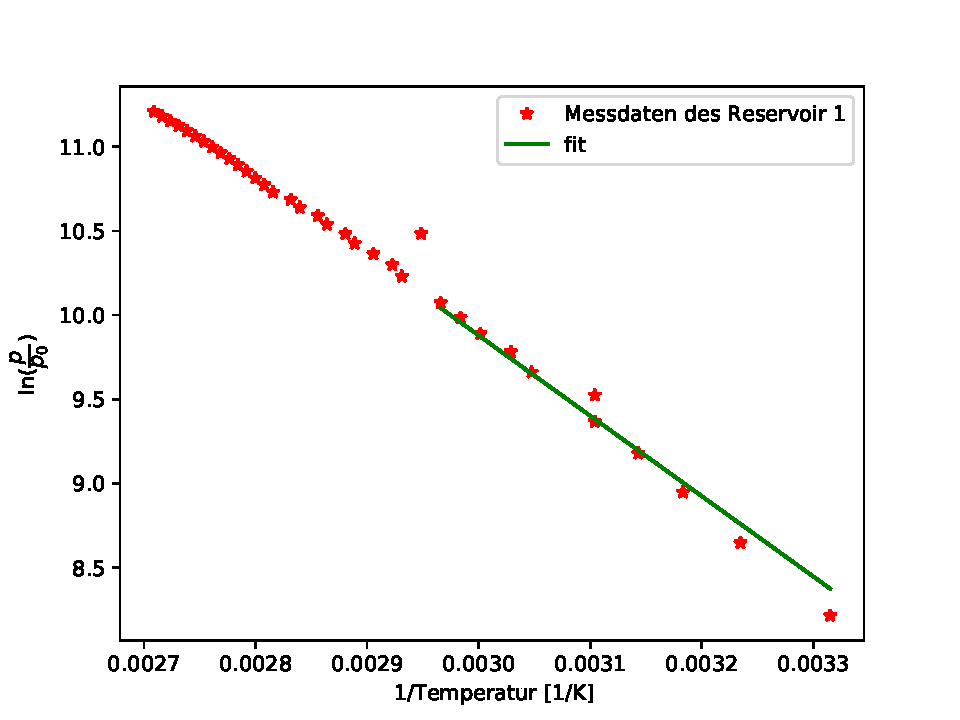
\includegraphics{plot1.pdf}
   \caption{Messwerte im Hochdruckbereich}
   \label{fig:plot1}
  \end{figure}
  \noindent Wie in Abbildung \ref{fig:plot1} bereits dargestellt, können die Messwerte durch ein Polynom
  der Form $p = a \cdot T³ + b \cdot T² + c \cdot T + d$ genähert werden. Die mit Python
  ermittelten Koeffizienten lauten:
  \begin{align*}
    & a = -0.5015 \pm 0.3859 \ \dfrac{Pa}{K³}\\
    & b = 750.5024 \pm 479.7916 \ \dfrac{Pa}{K²}\\
    & c = (-3.5129 \pm 1.9861) \cdot 10⁵ \ \dfrac{Pa}{K}\\
    & d = (5.269 \pm 2.7371) \cdot 10⁷ \ Pa\\
  \end{align*}
  Die Verdampfungswärme L lässt sich bekanntermaßen aus der Clausius-Clapeyron Gleichung 
  \begin{equation}
    \label{eqn:ccg}
    (V_D-V_F)dp = \dfrac{L}{T}dT \Leftrightarrow L = (T \cdot \dfrac{dp}{dT}\cdot(V_D-V_F)) 
  \end{equation}
  berechnen.
  Die Ableitung des Drucks nach der Zeit betraägt offensichtlich $\dfrac{dp}{dT}= 3a \cdot
  T²+2b\cdot T+ c$. $V_F$ kann hier erneut vernachlässigt werden.
  Da hier zu hoher Druck herrscht, um von einem idealen Gas ausgehen zu können, wird 
  $V_D$ anhand der Gleichung
  \begin{equation*}
  (p+\dfrac{a}{V²})V = RT \Leftrightarrow V = \dfrac{RT}{2p} \pm \sqrt{\dfrac{R²T²}{4p²}-\dfrac{a}{p}}
  \end{equation*}
  bestimmt. Eingesetzt in Gleichung \ref{eqn:ccg} ergibt sich für die Verdampfungswärme:
  \begin{equation*}
  L = T \cdot \dfrac{dp}{dT} \cdot (\dfrac{RT}{2p} \pm \sqrt{\dfrac{R²T²}{4p²}-\dfrac{a}{p}})
  \end{equation*}
  Aus dieser Gleichung ergeben sich zwei unterschiedliche Kurven für die Verdampungswärme, die
  Folgenden dargestellt sind. Abbilgung \ref{fig:plot2} behandelt den Fall, dass die Wurzel aufaddiert wird; 
  Abbildung \ref{fig:plot3} den Fall, dass die Wurzel subtrahiert wird.
  \begin{figure}[H]
   \centering
   \includegraphics{plot2.pdf}
   \caption{Verdampfungswärme mit positiver Wurzel}
   \label{fig:plot2}
  \end{figure}
  
  \begin{figure}[H]
   \centering
   \includegraphics{plot3.pdf}
   \caption{Verdampfungswärme mit negativer Wurzel}
   \label{fig:plot3}
  \end{figure}

  
  







